%        File: pyne_ans.tex 
%     Created: 6.28.2012 

\documentclass{anstrans}
%%%%%%%%%%%%%%%%%%%%%%%%%%%%%%%%%%%
\title{PyNE : Python For Nuclear Engineering}
\author{Anthony~M.~Scopatz$^1$, Paul~K.~Romano$^2$, Paul~P.H.~Wilson$^3$, Kathryn~D.~Huff$^3$}

%% uncomment these next five only if using anstrans
\institute{$^1$ University of Chicago, $^2$ Massachusetts Institute of Technology, $^3$ University of Wisconsin }
\email{pyne-dev@googlegroups.com}
\usepackage{graphicx}
\usepackage{booktabs} % nice rules for tables
\usepackage{microtype} % if using PDF
\newcommand{\units}[1] {\:\text{#1}}%
\newcommand{\SN}{S$_N$}%{S$_\text{N}$}%{$S_N$}%

\date{}
%%%%%%%%%%%%%%%%%%%%%%%%%%%%%%%%%%%
\begin{document}
%%%%%%%%%%%%%%%%%%%%%%%%%%%%%%%%%%%%%%%%%%%%%%%%%%%%%%%%%%%%%%%%%%%%%%%%%%%%%%%%
\section{Introduction}

PyNE, or `Python for Nuclear Engineering'\footnote{http://pyne.github.com}, is a
nascent free and open source C++/Cython/Python package for performing common
nuclear engineering tasks.  This is intended as a base-level tool kit - akin to
SciPy or Biopython - for common algorithms inside of the nuclear science and
engineering domain.

\section{Background}

While PyNE may be considered long overdue from an external perspective, the 
nuclear industry poses a uniquely high barrier to entry for free software.  
That closed source solutions are often easier to develop is an irony that 
increases the novelty of this package.

An initial hurdle for PyNE is the myriad of arcane file formats (both plain text
and binary) which have been industry standard since the 1960s.  Though obtuse 
specifications are not solely a nuclear problem, the scale of the number of formats 
is much greater.  Partly to blame is that some of these formats were enshrined 
in international law at a time when Fortran 2 was the language of choice.

Thus the emerging value of PyNE is that it allows new users to shortcut the tedious and 
error prone process of writing their own tools to parse these obtuse data and output file 
formats.  The current unfortunate state of affairs is due in part to huge institutional 
inertia on the part of the maintainers of such formats.  This manifests as a reluctance to 
develop or refactor new and existing codes in a modern open source manner.  PyNE seeks to 
gain human efficiency via a shared set of solutions rather than having every developer 
around the world replicate the same parsing routines.

Another major challenge for the community of PyNE developers is maintaining
the BSD license while explicitly avoiding any code which may be subject to 
export control.  Many nuclear engineering codes are open source in the sense
that the source code is distributed to developers who are then free to modify it.
However, due to the fear of illicit use for the development of weapons, these
same codes are then heavily export controlled and redistribution in any form is 
against their licenses and is likely illegal.

Redistribution concerns are not limited to source code.  Basic nuclear data, 
while fundamentally un-copywritable under Western jurisprudence, also 
be considered sensitive and subject to export control laws.  PyNE has developed
a three-tiered strategy to alleviate the data burden of the individual user based 
on the level of openness of the data. 

In spite of the above administrative concerns, PyNE's place in the nuclear ecosystem
requires it have a general architecture.  Large portions of the code base are 
written in pure C or C++ and are built as Python-independent shared libraries. This
enables other, compiled nuclear engineering codes to leverage PyNE.  Hence, the 
Cython layer has wrappers for C++ standard library containers (maps, 
sets, lists, etc) which implement the ``collections'' interface of the 
appropriate type.  Because of the high degree of factorization in PyNE, these wrappers 
could easily be reused by other projects.

%%%%%%%%%%%%%%%%%%%%%%%%%%%%%%%%%%%%%%%%%%%%%%%%%%%%%%%%%%%%%%%%%%%%%%%%%%%%%%%%
\section{Description of The Actual Work}

\textbf{WE SHOULD PUT SOME ACTUAL DISCUSSION OF PyNE CAPABILITIES HERE} This
talk will contain an overview of the current capabilities of PyNE, a discussion
of the export control issues, a related discussion on the redistribution of raw
nuclear data, and how the PyNE team has been successful in developing highly
performant tools for themselves and.

\subsection{NJOY Module}

Recently, the developers of PyNJOY, a set of Python bindings for processing
nuclear data using NJOY, agreed to have their work integrated with the PyNE
project as a new NJOY module. This will help to encourage active development and
wider participation in the project.

The NJOY module provides a simple method of generating nuclear data in a variety
of formats from raw ENDF data without the user having to worry about the exact
format of the NJOY input files. Thus, with a single Python script, it is
possible to process tens of hundreds of nuclides at once rather than managing
many NJOY input files.

\subsection{ACE Module}

One of the most common data formats used to represent pointwise
linearly-interpolable cross sections is the ACE (A Compact ENDF) format. This
format was introduced by LANL for use in the MCNP \cite{mcnp} code and is now
used by the Serpent \cite{serpent} and OpenMC \cite{openmc} Monte Carlo codes as
well. While there are a variety of resources that allow a user to inspect and
plot data directly from ENDF, there has generally been no good means of looking
at processed data in the ACE format that is actually used in Monte Carlo
simulations. As such, a module has been added to PyNE to parse and store data
from ASCII or binary ACE files. A front-end graphical user interface is also in
development that will give the user an easy interface to view and compare both
cross sections and secondary energy and angle
distributions. Figure~\ref{fig:ace-gui} shows cross section data for Pu-239
being plotted within the GUI.
\begin{figure}[ht]
  \centering
  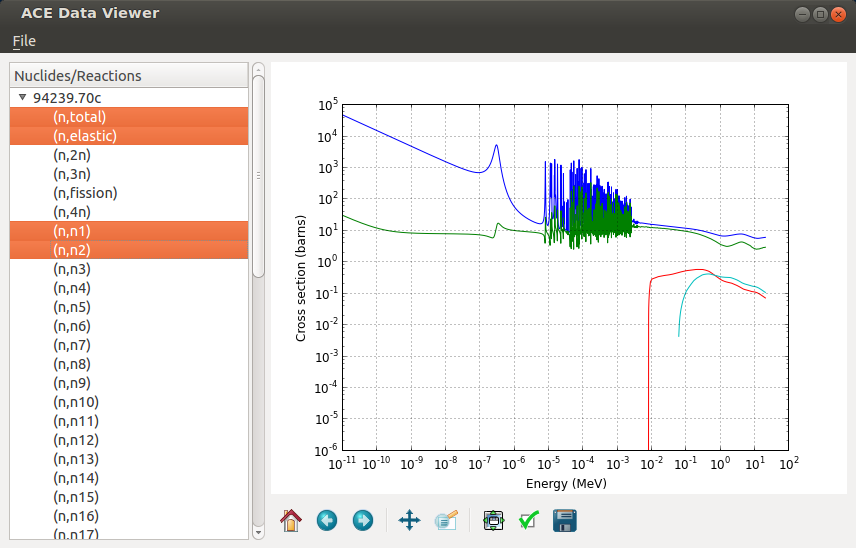
\includegraphics[width=3.3in]{ace-gui.png}
  \caption{Front-end graphical user interface for plotting ACE format data in
    PyNE.}
  \label{fig:ace-gui}
\end{figure}

%%%%%%%%%%%%%%%%%%%%%%%%%%%%%%%%%%%%%%%%%%%%%%%%%%%%%%%%%%%%%%%%%%%%%%%%%%%%%%%%
\section{Conclusions}

%%%%%%%%%%%%%%%%%%%%%%%%%%%%%%%%%%%%%%%%%%%%%%%%%%%%%%%%%%%%%%%%%%%%%%%%%%%%%%%%
\nocite{*}
\bibliographystyle{ans}
\bibliography{pyne_ans2012}
\end{document}


